\documentclass[tikz,border=14pt]{standalone}
\usepackage{tikz}
\usetikzlibrary{positioning,calc,arrows.meta,fit}

\definecolor{paper}{RGB}{255,253,247}
\definecolor{ink}{RGB}{17,17,17}
\definecolor{muted}{RGB}{95,90,82}
\definecolor{arcface}{RGB}{244,170,75}
\definecolor{dino}{RGB}{87,142,201}
\definecolor{convnext}{RGB}{98,168,126}
\definecolor{fusion}{RGB}{198,151,215}
\definecolor{regressor}{RGB}{230,218,132}
\definecolor{output}{RGB}{235,118,118}

\tikzset{
  arrow/.style={-{Latex[length=3mm]}, line width=0.9pt, draw=ink},
  branch/.style={-{Latex[length=2.6mm]}, line width=0.85pt, draw=ink, opacity=0.82},
  label/.style={font=\sffamily\scriptsize, text=muted, align=center},
  title/.style={font=\sffamily\bfseries\small, text=ink, align=center},
  small/.style={font=\sffamily\scriptsize, text=ink, align=center},
}

% 3D-ish block: name, coordinate, width, height, color, title, subtitle
\newcommand{\Block}[7]{%
  \node[draw=ink, line width=0.7pt, fill=#5!74, minimum width=#3, minimum height=#4, align=center, inner sep=4pt] (#1) at #2 {\begin{tabular}{c}\textbf{#6}\\[-1pt]{\scriptsize #7}\end{tabular}};
  \path let \p1=($(#1.north east)-(#1.north west)$), \p2=($(#1.north east)-(#1.south east)$) in coordinate (#1-ne) at (#1.north east);
  \draw[draw=ink, line width=0.55pt, fill=#5!50] (#1.north west) -- ++(0.16,0.16) -- ($(#1.north east)+(0.16,0.16)$) -- (#1.north east) -- cycle;
  \draw[draw=ink, line width=0.55pt, fill=#5!42] (#1.north east) -- ++(0.16,0.16) -- ($(#1.south east)+(0.16,0.16)$) -- (#1.south east) -- cycle;
}

\begin{document}
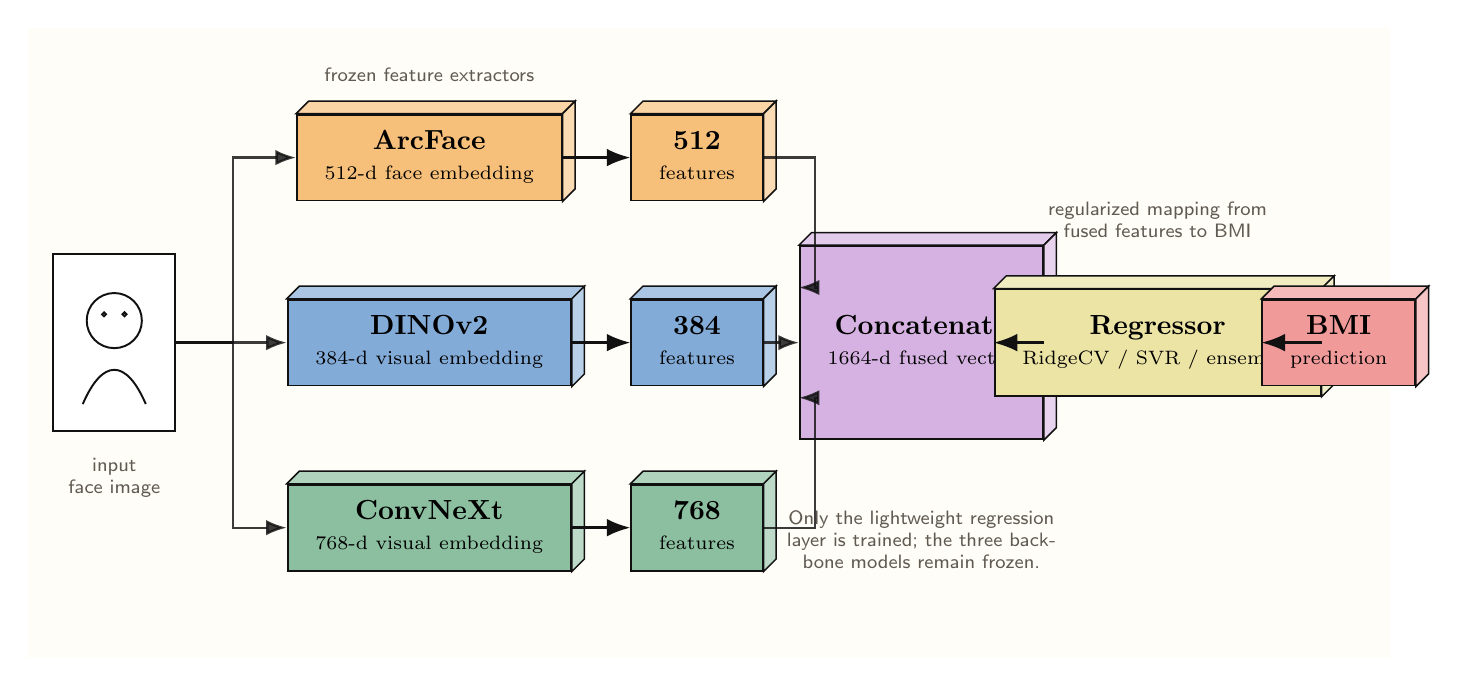
\begin{tikzpicture}[x=1cm,y=1cm]
  \fill[paper] (-1.1,-4.0) rectangle (16.2,4.0);

  % Input image panel
  \node[draw=ink, line width=0.8pt, fill=white, minimum width=1.55cm, minimum height=2.25cm] (img) at (0,0) {};
  \draw[ink, line width=0.7pt] ($(img.center)+(0,0.28)$) circle (0.35);
  \draw[ink, line width=0.7pt] ($(img.center)+(-0.13,0.36)$) circle (0.025);
  \draw[ink, line width=0.7pt] ($(img.center)+(0.13,0.36)$) circle (0.025);
  \draw[ink, line width=0.7pt] ($(img.center)+(-0.40,-0.78)$) .. controls ($(img.center)+(-0.15,-0.20)$) and ($(img.center)+(0.15,-0.20)$) .. ($(img.center)+(0.40,-0.78)$);
  \node[label, below=0.20cm of img] {input\\face image};

  % Frozen feature branches
  \Block{arc}{(4.0,2.35)}{2.45cm}{1.05cm}{arcface}{ArcFace}{512-d face embedding}
  \Block{dino}{(4.0,0)}{2.45cm}{1.05cm}{dino}{DINOv2}{384-d visual embedding}
  \Block{conv}{(4.0,-2.35)}{2.45cm}{1.05cm}{convnext}{ConvNeXt}{768-d visual embedding}

  \node[label, above=0.28cm of arc] {frozen feature extractors};

  % Feature-vector slabs
  \Block{avec}{(7.4,2.35)}{1.35cm}{0.78cm}{arcface}{512}{features}
  \Block{dvec}{(7.4,0)}{1.35cm}{0.78cm}{dino}{384}{features}
  \Block{cvec}{(7.4,-2.35)}{1.35cm}{0.78cm}{convnext}{768}{features}

  % Fusion and regressor
  \Block{cat}{(10.25,0)}{2.25cm}{2.45cm}{fusion}{Concatenate}{1664-d fused vector}
  \Block{reg}{(13.25,0)}{2.10cm}{1.35cm}{regressor}{Regressor}{RidgeCV / SVR / ensemble}
  \Block{bmi}{(15.55,0)}{1.20cm}{1.05cm}{output}{BMI}{prediction}

  % Connections
  \draw[branch] (img.east) -- ++(0.72,0) |- (arc.west);
  \draw[branch] (img.east) -- (dino.west);
  \draw[branch] (img.east) -- ++(0.72,0) |- (conv.west);

  \draw[arrow] (arc.east) -- (avec.west);
  \draw[arrow] (dino.east) -- (dvec.west);
  \draw[arrow] (conv.east) -- (cvec.west);

  \draw[branch] (avec.east) -- ++(0.65,0) |- ($(cat.west)+(0,0.70)$);
  \draw[branch] (dvec.east) -- (cat.west);
  \draw[branch] (cvec.east) -- ++(0.65,0) |- ($(cat.west)+(0,-0.70)$);

  \draw[arrow] (cat.east) -- (reg.west);
  \draw[arrow] (reg.east) -- (bmi.west);

  % Notes
  \node[label, below=0.78cm of cat, text width=5.1cm] {Only the lightweight regression layer is trained; the three backbone models remain frozen.};
  \node[label, above=0.52cm of reg, text width=3.2cm] {regularized mapping from fused features to BMI};
\end{tikzpicture}
\end{document}
